\clearpage
\chapter{Conclusion and Outlook}\label{ch:futureimp}

Section \ref{sec:2Dcase} shows the reconstruction of projected electron density using \Bmq as a constraint. It is shown that by combining phasing algorithm with the constraint on \Bmq  the electron density converges into the original model. Another important treatmant in the method is to use Fourier transform in polar coordinate. The definition of \Bmq is described in polar coordinate, then the loss of information due to the interpolation is minimal throughout the iteration in phasing. For that reason, the new phasing algorithm in terms of polar coordinate is developed in section \ref{sec:2Dcase}.     

The important constraint that is shown in section \ref{sec:2Dcase} is only constraining to the diagonal value of \Bmq. Beside the diagonal value, the nondiagonal value can have important information, which can be used as the phasing constraint. In the equation \ref{eq:Bmqdef}, the only missing information from \Bmq to $I_{m}(q)$ is only the phase for each $m$. Hence, there is only one unique information that is unknown. 

It is suggested that SVD on the matrix \Bmq will only have one singular value because the matrix \Bmq is a dot product of vector $I_{m}(q)$ with only the phase missing. The SVD can reveal the independent parameter to describe the data. Thus, there will be one singular value of \Bmq because the independent parameter is only the phase of $I_{m}(q)$. Thus, the previous method in section \ref{sec:2Dcase} can be improved by constraining the nondiagonal value of \Bmq. The expected reconstruction should be much better if the nondiagonal value or SVD is used as a constraint in polar phasing algorithm.  


In section \ref{sec:triple} the use of triple correlation as additional information to reconstruct electron density is discussed. The derivation of triple correlation is given from equation \ref{eq:crosstripcor} to equation \ref{eq:triple}. Because of the complexity of the triple correlation, it is used only for signs determination. 

The simulation shows that triple correlation and pair correlation can be used to reconstruct electron density from the object that has azimuthal symmetry. By imposing the azimuthal symmetry, only $m=0$ is nonzero in spherical harmonics expansion. Thus, the magnitude of \Ilm can be obtained directly from the diagonal value of \Blq. As a result of that, only sign of \Ilm is nonunique and need to be determined from the different information other than \Blq. The nonuniqueness is resolved by try different signs combination and fit them to the triple correlation. The set of signs, which is closest to the triple correlation, is taken as the correct combination of the sign. Consequently, the diffraction volume can be constructed from \Ilm and the electron density is obtainable using phasing algorithm. This conclude section \ref{sec:triple} where the triple correlation and pair correlation can be used to reconstruct the electron density from the random angle diffraction patterns. 

The explanation and result of how the information about symmetry is obtained from pair correlation are given in section \ref{sec:pattsymm}. Currently, two quantities are used to differentiate the symmetry of the object. Those are the selection rule explained in section \ref{icosph} and PCA, which is explained in section \ref{sec:PCA}. The selection rule is used to differentiate icosahedral symmetry and azimuthal symmetry whereas PCA is used to differentiate azimuthal symmetry, $C_n$, and asymmetry. The selection rule and PCA complement each other to differentiate the subset of the symmetry. The method suggests that the information of symmetry is not just a mere assumption but also information obtainable from the experiment.

The symmetry determination, which uses the method, requires understanding of the spherical harmonics selection rule and the lowest number of independent parameters of its spherical harmonics expansion. It is possible to extend the determination of the other type symmetry as long as the selection rule and the lowest number of independent parameters are provided. Additionally, currently there is no relation that describe the uniqueness of the symmetry determination. The study of the uniqueness of PCA and the symmetry will complement the theory which I developed.      

Another discussion that is described in section \ref{sec:pattsymm} is the limit of the method. Currently, the inversion symmetry cannot be determined using PCA. The inversion symmetry always exist in reciprocal space. Moreover, the method uses reciprocal space to deduce the symmetry of the object indirectly. As a result of that, the existance of the inversion symmetry of the electron density cannot be determined using method described in section \ref{sec:pattsymm}.

Another application of PCA or SVD of \Blq is discussed as well. Beside symmetry determination, PCA can be used to check the convergence of \Blq. Section \ref{sec:convlim} explains that some number of diffraction patterns is needed to get the convergence of \Blq. The test that is explained is to check the number of nonzero singular values of \Blq. There is a maximum number of singular values of \Blq if the \Blq converges into a form of dot product. The number is ($2l+1$), which is the number of singular values for asymmetric structure. Any structure theoretically cannot have more number of singular values more than ($2l+1$) because the number of independent parameters to describe asymmetric structure is ($2l+1$). In conclusion, if the SVD \Blq give the number of singular values more than ($2l+1$) then the \Blq doesn't converge.  
   
Section \ref{sec:posconst} explains the reconstruction of the electron density by using pair correlation and positivity constraint. The method uses SVD to get the estimation of \Ilm. The missing or nonunique information is the orthogonal matrix. The orthogonal matrix is determined by imposing the intensity to be positive number. The method defines an objective function in which if it is zero then the orthogonality is satisfied. The active set algorithm is used to find the zero objective function and at the same time satisfy the positivity constraint. In conclusion, the diffraction volume can be obtained and the electron density is obtained using phasing algorithm.  

Currently, the output of the reconstruction is still low resolution reconstruction. The reason for that because there is still a separate step between reconstructing the diffraction volume and the phasing to get electron density. The better reconstruction will be obtained by combining those steps. In other words, it adds additional constraint beside positivity. The constraint comes from any phasing constraint in real space. 

Since equation \ref{eq:IqtoOrtho} relates the intensity to the $O^{l}_{mm'}$ directly, it is possible to use the relation as additional step in phasing algorithm. It is shown in figure \ref{fig:phasmo} how it is done. It involves finding the closest orthogonal matrix or what is known as procrustes problem.   
\begin{figure}[h!]
  \centering
  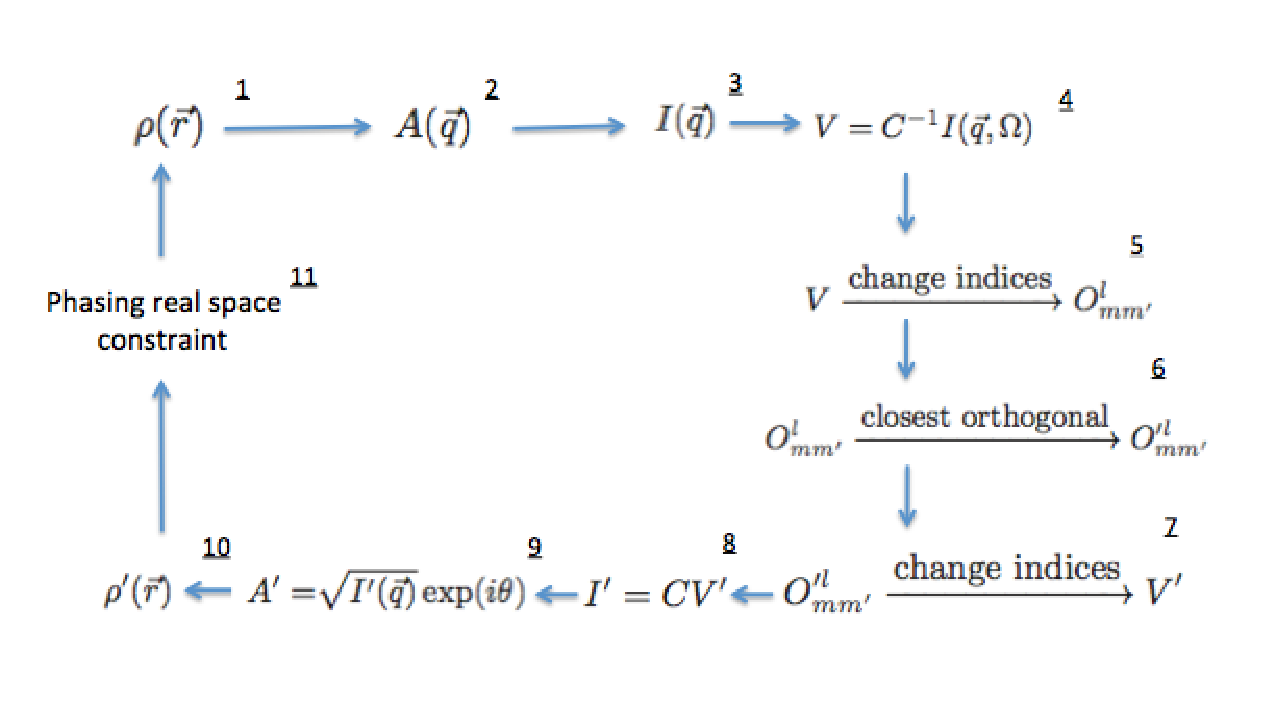
\includegraphics[width=.8\textwidth]{fucycle}
\caption{Modified phasing algorithm which find closest orthogonal matrix}
\label{fig:phasmo}
\end{figure}
\begin{enumerate}
  \item Start initial guess of $\rho(\vec{r})$. 
  \item Use FFT to calculate $A(\vec{q})$. 
  \item $I(\vec{q})=|A(\vec{q})|^{2}$ and keep information of phase. 
  \item Estimation of vector $V$ is obtained based on equation \ref{eq:IqtoOrtho}. 
  \item Change from 1D index of vector $V$ into 3D index of matrix $O^{l}_{mm'}$ for each $l$. 
  \item Find closest orthogonal matrix or it is known as procrustes problem. 
  \item Change from 3D index of matrix $O^{l}_{mm'}$ for each $l$ into 1D index of vector $V$.
  \item Use equation \ref{eq:IqtoOrtho} to obtain next estimation of vector $V$.
  \item Calculate $A(\vec{q})$ from previous information of phase. 
  \item Use inverse FFT to obtain $\rho(\vec{q})$. 
  \item Use HIO, ER, shrinkwrap, or charge-flipping to constraint $\rho(\vec{r})$ and cycle is repeated.
\end{enumerate}

The method described above combines the phasing algorithm and the SVD of \Blq into one iteration. By having it into one iteration, the additional information is obtained from the phasing constraint such as the electron density has to be positive. Thus, it is expected to have a better reconstruction compare to the method that only use positivity constraint.  
